\documentclass[11pt,a4paper]{article}

% ----- Packages -----
\usepackage[utf8]{inputenc}
\usepackage[T1]{fontenc}
\usepackage[english]{babel}
\usepackage{amsmath,amssymb,amsthm}
\usepackage{booktabs}
\usepackage{array}
\usepackage{graphicx}
\usepackage[table]{xcolor}
\usepackage{hyperref}
\usepackage{geometry}
\usepackage{caption}
\usepackage{enumitem}
\usepackage[expansion=false,protrusion=true]{microtype}
\usepackage{tikz}
\usetikzlibrary{positioning,arrows.meta,shapes,fit,backgrounds,calc}
\usepackage{listings}
\usepackage{textcomp}
\usepackage{relsize}

\geometry{margin=2.5cm}

% ----- Source-Code Listings -----
\lstset{
    basicstyle=\ttfamilyfootnotesize,
    keywordstyle=\color{blue!60!black},
    commentstyle=\color{green!50!black},
    stringstyle=\color{red!60!black},
    showstringspaces=false,
    breaklines=true,
    frame=single,
    numbers=left,
    numberstyle=\tiny\color{gray},
    captionpos=b,
}

% ----- Theorem Environments -----
\newtheorem{theorem}{Theorem}
\newtheorem{lemma}[theorem]{Lemma}
\newtheorem{proposition}[theorem]{Proposition}
\theoremstyle{definition}
\newtheorem{definition}{Definition}
\newtheorem{remark}{Remark}

% ----- Captions -----
\captionsetup{labelfont=bf}

% ----- Title -----
\title{\textbf{Regime-Preserving Bootstrap for\\FX Fair-Value Models}}

\author{David Vossebürger\\
\small Independent Researcher\\
\small \texttt{david.vossebuerger@proton.me}}

\date{June 2026}

\begin{document}

\maketitle

\begin{abstract}
\noindent
This paper documents a regime-preserving bootstrap procedure for validating the out-of-sample robustness of FX fair-value strategies (BEER, FEER, PPP). The central idea is that standard bootstrap methods (IID, Moving Block, Stationary Block) destroy the economic regime structure of macro-FX data and thereby systematically bias Sharpe ratio inference. We propose two regime-aware resamplers -- Regime-Uniform (block resampling within macro-regimes) and Regime-Markov (block resampling with calibrated Markov transition matrix) -- and validate them using five structure metrics, a Sharpe loss metric, an arrangement distance, a stationarity gate per Section~11.7, and Wilcoxon paired tests with Benjamini-Hochberg FDR.

Applied to a BEER pricer for three currency pairs (EURUSD, GBPUSD, USDJPY) with $B = 1999$ bootstrap replicates, the key finding is: \emph{Regime-Markov reduces the bootstrap Sharpe loss by a factor of $1.3\times$ compared to Regime-Uniform (the simpler block resampler without transition structure) and by a factor of $4.6\times$ compared to the naive IID benchmark}. The Markov transition structure provides the additional gain over pure block resampling. The calibrated transition matrix passes the Section~11.7 stationarity gate (TV drift $= 0.10$), validating forward projections over short horizons of $\sim$3--5 Markov steps. We document the complete metric definitions, the implementation, and the honest limits of cross-pair generalization.
\end{abstract}

\tableofcontents
\newpage

%==========================================================
\section{Introduction}
%==========================================================

The out-of-sample validation of FX fair-value strategies (BEER, FEER, PPP) requires a statistical test that preserves the \emph{macroeconomic regime structure} of the underlying data. Standard block bootstrap methods (Moving Block, Stationary Block) preserve the temporal dependence within a block, but they do not preserve the \emph{identity} of the regime: a simulated path that draws an observation from 2009 immediately followed by an observation from 2021 has no economic meaning, and its Sharpe value is not interpretable.

This paper documents the implementation, metrics, and validation of a regime-preserving bootstrap family for FX fair-value backtests. The core idea is to view the empirical macro-FX history as a sequence of \emph{regime blocks} -- periods of coherent monetary policy and macroeconomic fundamentals -- and resample at the block level rather than the observation level. Two variants are proposed:

\begin{itemize}[leftmargin=2em]
  \item \textbf{Regime-Uniform}: Resampling entire regime blocks uniformly with replacement; regime identity is preserved, the transition structure between regimes is lost.
  \item \textbf{Regime-Markov}: Resampling entire regime blocks via a calibrated Markov chain; both regime identity and transition structure are preserved.
\end{itemize}

The overall method is compared to three baselines: IID, Moving Block Bootstrap (MBB), and Stationary Block Bootstrap (SB). The performance gap is measured on six loss levels (L0--L4) plus an arrangement distance (Spec Section~6) and a stationarity gate (Spec Section~11.7).

The contributions of this paper are:
\begin{enumerate}[leftmargin=2em]
  \item A complete, code-validated metric suite for regime-aware bootstrap validation (Section~\ref{sec:metrics}).
  \item A soft-whitelist Sinkhorn-Knopp calibration algorithm for the Markov transition matrix (Section~\ref{sec:transition}).
  \item Empirical results on three currency pairs (EURUSD, GBPUSD, USDJPY) showing that Regime-Markov simultaneously dominates the L0 family and the temporal structure metrics (Section~\ref{sec:results}).
  \item A documented list of remaining limitations (Section~\ref{sec:limits}), the most important being that the upstream pipeline of the BEER pricer is not yet fully pair-aware.
\end{enumerate}

The rest of the paper is organized as follows. Section~\ref{sec:method} briefly recapitulates the bootstrap methods. Section~\ref{sec:metrics} provides the complete metric definitions -- this is the methodological heart of the paper. Section~\ref{sec:transition} describes the transition matrix calibration. Section~\ref{sec:decision} formulates the Spec-Section~5 decision rule. Section~\ref{sec:implementation} covers the code structure. Section~\ref{sec:data} describes the data and the regime taxonomy. Section~\ref{sec:results} reports the empirical findings. Section~\ref{sec:limits} discusses the limitations. Section~\ref{sec:concl} concludes.

%==========================================================
\section{Methodology (compact)}
\label{sec:method}
%==========================================================

The complete method is specified in the project specification document (``Regime-Preserving Bootstrap for FX Fair-Value Models''); we only recapitulate the essentials below.

\subsection{Regime Taxonomy}

We use an expert-defined taxonomy of 8 EUR/USD macro-monetary regimes from 2003 to today:
\begin{enumerate}[leftmargin=2em]
  \item PRE\_GFC (2003-01 $\to$ 2008-08, 68 months)
  \item GFC (2008-09 $\to$ 2009-06, 10 months)
  \item EURO\_CRISIS\_ERA (2009-07 $\to$ 2012-08, 38 months)
  \item TAPER\_TRANSITION (2012-09 $\to$ 2014-05, 21 months)
  \item NIRP\_DOVISH (2014-06 $\to$ 2019-12, 67 months)
  \item COVID (2020-01 $\to$ 2021-12, 24 months)
  \item INFLATION\_SHOCK (2022-01 $\to$ 2023-09, 21 months)
  \item DISINFLATION (2023-10 $\to$ today, $\sim$39 months)
\end{enumerate}
These definitions are \emph{purely macroeconomic}: they are derived from ECB and Fed policy regime shifts, not from FX price data, to avoid look-ahead bias in the bootstrap.

\subsubsection*{Notation and Setup}

We collect the symbols used throughout the paper here. Time-indexed
quantities are denoted with subscript $t$; regime indices with
$i,j \in \{1, \ldots, K\}$ (default $K = 8$); methods with
$m \in \{\text{IID, MBB, SB, Regime-Uniform, Regime-Markov}\}$.

\begin{itemize}[leftmargin=2em]
  \item $X_t \in \mathbb{R}^d$ --- multivariate monthly feature vector
        ($d=5$: InflationDiff, RealRateDiff, GDPDiff, RealVol, Carry).
  \item $B_k$ --- the $k$-th regime block, $B_k = \{X_t : t \in I_k\}$
        for index set $I_k \subseteq \{1, \ldots, T\}$.
  \item $P \in \mathbb{R}^{K \times K}$ --- Markov transition matrix
        with $P_{ij} = \Pr(\text{regime } j \text{ at } t+1 \mid \text{regime } i \text{ at } t)$.
  \item $\pi(P) \in \mathbb{R}^K$ --- stationary distribution of $P$.
  \item $S_m^{(b)}$ --- Sharpe ratio of the $b$-th bootstrap replicate
        under method $m$, $b = 1, \ldots, B$ ($B = 1999$).
  \item $S^{\text{obs}}$ --- observed (in-sample) Sharpe ratio.
  \item $L_k^{(m)}(P^{\star}, P)$ --- generic loss metric on
        $(P^{\star}, P)$ for method $m$ and level $k$ ($k = 0, \ldots, 3$).
\end{itemize}

For convenience, $L_k$ always denotes a \emph{lower-is-better} loss
between an empirical object and its bootstrap-replicated counterpart;
the unit of each loss depends on the metric and is documented in
its definition. The \emph{family-level} L0 test asks whether
Regime-Markov dominates all three baseline methods (IID, MBB, SB)
on L0 \emph{simultaneously}; this is a binary decision that does not
depend on $p$-values.

\subsubsection*{Toy Example: A 2-Regime Chain}

To build intuition before the formal exposition, consider a minimal
toy example with $K=2$ regimes, observed for $T = 4$ periods
($A \to B \to A \to B$). The empirical transition counts are
$N_{12} = N_{21} = 2$, the row-normalized empirical transition
matrix is $\hat P = \begin{pmatrix} 0 & 1 \\ 1 & 0 \end{pmatrix}$, and
the empirical regime frequencies are $\hat\pi = (0.5, 0.5)$.
Regime-Markov with the empirical $\hat P$ produces alternating
sequences $A B A B \ldots$, exactly the only sequence the data
support. IID and Regime-Uniform also produce $ABAB$ sequences
(they happen to coincide with the empirical transitions), but for
$K=3$ or $K=8$ the three methods diverge and Regime-Markov is the
only one that respects the long-run transition structure.

This toy example is used informally throughout the paper to
illustrate the mechanism. The full empirical results with
$K = 8$ and $T \approx 280$ months are reported in
Section~\ref{sec:results}.

\subsection{Bootstrap Methods}

Let $\{X_t\}_{t=1}^{T}$ be the monthly FX time series, partitioned into $K=8$ regime blocks $B_1, \ldots, B_K$ with $B_k = \{X_t : t \in I_k\}$ for index sets $I_k$. The five resampling methods are:

\begin{definition}[IID]
$X_t^{\star} \stackrel{\text{iid}}{\sim} \hat{F}$, where $\hat{F}$ is the empirical distribution of $\{X_t\}$. This is the textbook bootstrap; it destroys all temporal structure.
\end{definition}

\begin{definition}[Moving Block Bootstrap (MBB)]
Choose block length $\ell$, partition the data into overlapping blocks of length $\ell$, draw blocks i.i.d.\ uniformly with replacement, and concatenate. MBB preserves short-range temporal dependence within each block, but does not respect regime identity.
\end{definition}

\begin{definition}[Stationary Block Bootstrap (SB)]
Like MBB, but with random block length drawn from a geometric distribution; this breaks the artificial periodicity of MBB. Also regime-agnostic.
\end{definition}

\begin{definition}[Regime-Uniform]
Resampling entire regime blocks uniformly with replacement and concatenation. Regime identity is preserved within each block, but the transition structure between regimes is destroyed.
\end{definition}

\begin{definition}[Regime-Markov]
Resampling entire regime blocks via a Markov chain: draw the first regime from the initial distribution, iterate according to the calibrated transition matrix $P$, and concatenate the corresponding blocks. Both regime identity and transition structure are preserved.
\end{definition}

The number of bootstrap replicates is consistently $B = 1999$. The initial distribution of Regime-Markov corresponds to the empirical distribution of the first block; the transition matrix is estimated from the empirical block sequence and calibrated via the algorithm in Section~\ref{sec:transition}.

\subsection{Pricer: BEER (background)}

For the L0 Sharpe loss metric, we use the BEER pricer (Behavioural Equilibrium Exchange Rate) by Clark and MacDonald (1998) in its FMOLS implementation:
\[
\ln Q_t = \alpha + \beta_1\, \text{TOT}_t + \beta_2\, \text{NFA}_t
+ \beta_3\, (\text{ProdDiff})_t + \beta_4\, (\text{RateDiff})_t
+ \varepsilon_t,
\]
estimated via OLS with Newey-West HAC standard errors. The fair-value gap $g_t = \ln Q_t - \widehat{\ln Q}_t$ drives a mean-reversion position; the strategy Sharpe is $\bar{g}/\sigma_g \cdot \sqrt{4}$ (quarterly annualization). BEER is \emph{order-sensitive}: permuting the order of returns changes the realized Sharpe through the serial correlation of the gap. This makes BEER the discriminating pricer for the L0 test; an order-invariant pricer (e.g.\ a simple fair-value gap mean-reversion) would by construction tie at L0.

%==========================================================
\section{Metrics}
\label{sec:metrics}
%==========================================================

The metric suite is the methodological core of the paper. We define five loss levels L0--L4 plus an arrangement distance and a stationarity gate. The naming is consistent with the project specification document; the rationale for each metric is given below.

\subsection{L0: Sharpe Loss (Family Test)}

\begin{definition}[L0 (Sharpe Loss)]
For a bootstrap method $m$, let $\{\widehat{S}^{\star (b)}\}_{b=1}^{B}$ be the bootstrap replicates of the strategy Sharpe. The L0 loss is
\[
L_0^{(m)} \;=\; \mathbb{E}\bigl[|\widehat{S}^{\star} - S|\bigr]
\;=\; \frac{1}{B}\sum_{b=1}^{B}
\bigl|\widehat{S}^{\star (b)} - S\bigr|,
\]
where $S$ is the original (in-sample) Sharpe.
\end{definition}

\begin{proposition}[Why L0]
If a bootstrap method destroys the dependence structure of the returns, the simulated Sharpe is biased: typically inflated (because the destroyed serial correlation deflates the Sharpe ratio denominator). L0 is the natural measure of how far \emph{this particular bootstrap world} deviates from the original in Sharpe terms.
\end{proposition}

\begin{proposition}[Family-L0 PASS criterion]
A bootstrap method $m$ achieves \emph{family-L0 PASS} if
\[
L_0^{(m)} \;<\; \min\bigl\{
L_0^{(\text{IID})},\, L_0^{(\text{MBB})},\, L_0^{(\text{SB})}
\bigr\}.
\]
In words: the candidate method must beat all three naive
baselines (IID, MBB, SB) on L0 \emph{simultaneously}. A tie with
one baseline (within $\text{SE}(\text{Sharpe})$) is acceptable; a
loss against any baseline is a fail.
\end{proposition}

\begin{remark}[Why a binary criterion, not a $p$-value]
Family-L0 PASS is a deterministic decision: did the method
dominate, or didn't it? It does not depend on per-test $p$-values.
We report $p$-values from the paired sign test (Section~\ref{sec:limits})
to \emph{quantify} the statistical confidence in the effect size
(L0/IID = $4.6\times$, L0/Uniform = $1.3\times$), not to decide
whether the family criterion holds.
\end{remark}

\textbf{Normalization.} We report $L_0 / \text{SE}(\text{Sharpe})$ with $\text{SE}(\text{Sharpe}) = \sqrt{(1 + 0.5\,S^2)/T}$ (Lo, 2002). This yields a scale-free measure: an L0 of $0.14$ at $\text{SE} = 0.11$ means that a typical bootstrap world lies $\sim$1.3 sample SDs from the original Sharpe. The alternative $L_0 / \sqrt{B}$ is the MC standard error of the mean and is much smaller ($\sim 0.0024$); we do \emph{not} report it.

\subsection{L1: Contemporaneous Correlation Loss}

\begin{definition}[L1 (Correlation Loss)]
Let $\hat{\rho}$ be the empirical correlation matrix of the 7 HMM input features over the original series, and $\hat{\rho}^{\star}$ the corresponding matrix in the bootstrap world. The L1 loss is
\[
L_1 \;=\; \|\hat{\rho} - \hat{\rho}^{\star}\|_F,
\]
the Frobenius norm of the correlation matrix difference.
\end{definition}

\textbf{Caveat.} IID, MBB, and SB preserve contemporaneous correlation by construction. L1 therefore discriminates poorly between bootstrap variants. We report it for completeness.

\subsection{L2: Wasserstein Distance}

\begin{definition}[L2 (Wasserstein Loss)]
Let $\hat{F}$ be the empirical joint distribution of the 7 features in the original series and $\hat{F}^{\star}$ the corresponding distribution in the bootstrap world. The L2 loss is the 2-Wasserstein distance
\[
L_2 \;=\; W_2(\hat{F},\, \hat{F}^{\star}).
\]
\end{definition}

$W_2$ measures the minimal transport costs between the two distributions. It is sensitive to differences in both the marginal distributions and the dependence structure, and penalizes any block-shuffling operation that changes the joint form.

\subsection{L3: Network / Spectral Structure}

We report two L3 variants. They differ in the matrix $M$ whose distance is measured.

\begin{definition}[L3$_{\text{fro}}$ (Frobenius)]
Let $M$ be the transition-matrix-like joint adjacency of the HMM features and $M^{\star}$ its bootstrap counterpart. Then $L_3^{\text{fro}} = \|M - M^{\star}\|_F$.
\end{definition}

\begin{definition}[L3$_{\text{spec}}$ (Spectral)]
$L_3^{\text{spec}} = \sum_i |\lambda_i(M) - \lambda_i(M^{\star})|$, where $\lambda_i$ are the eigenvalues. The spectral loss is more sensitive to the global structure of the whole than the Frobenius loss; it rewards methods that preserve the eigenvalue spectrum of the empirical joint.
\end{definition}

\subsection{L4: Temporal Structure}

\begin{definition}[L4$_{\text{temporal}}$]
A composite of four temporal statistics, averaged over the replicates:
\begin{itemize}[leftmargin=2em]
  \item Lag-1 autocorrelation of FX returns,
  \item Lo-MacKinlay variance ratio at lag 12,
  \item Maximum drawdown of cumulative FX log returns,
  \item Lag-$k$ cross-correlation between FX returns and strategy position, for $k=1,2,3$.
\end{itemize}
The loss is the mean absolute difference of each statistic between original and bootstrap world.
\end{definition}

\begin{proposition}[L4 is construction-bounded]
For any block-level bootstrap method $m \in \{\text{IID, MBB, SB,
Regime-Uniform, Regime-Markov}\}$ that resamples entire regime
blocks without modifying their internal order, the temporal
structure $L_4$ of the bootstrap-replicated regime sequence is
\emph{preserved by construction}:
\[
L_4^{(m)} = 0 \quad \text{for all } m.
\]
\end{proposition}

\begin{remark}
L4 is therefore not a discriminating metric between block-level
methods. We report it as a sanity check (a non-zero L4 would
indicate a bug, not a real failure). The discriminating structure
metrics are L1, L2, and L3.
\end{remark}

\subsection{Arrangement Distance (Spec Section~6)}

The arrangement distance tests whether the bootstrap preserves the \emph{regime-sequence structure}. Two complementary metrics:

\begin{definition}[Composition Distance]
$L_{\text{comp}} = \sum_{k=1}^{K} |f^{\star}_k - f_k|$, where $f_k$ is the empirical frequency of regime $k$ in the original sequence and $f^{\star}_k$ in the bootstrap sequence. This is the $L_1$ distance of the regime frequency histograms.
\end{definition}

\begin{definition}[Transition Distance]
$L_{\text{trans}} = \sum_{i,j} |T^{\star}_{ij} - T_{ij}|$, the $L_1$ distance of the transition count matrices (row-normalized).
\end{definition}

(Note: The normalized edit distance $L_{\text{edit}}$ was deleted -- it correlates strongly with the transition distance and only doubled the attack surface without new information.)

The condition \emph{arrangement is FAR} (Spec Section~5) requires that the bootstrap sequence differs measurably from the original sequence on at least one of these three metrics. The transition distance is the most diagnostic (it directly measures whether the simulator preserved the regime-to-regime flow).

\subsection{Section~11.7 Stationarity Gate}

\begin{definition}[Stationarity Gate]
Let $P$ be the calibrated Regime-Markov transition matrix with stationary distribution $\pi(P)$ (the left eigenvector for eigenvalue 1). Let $\hat{\pi}$ be the empirical regime frequency vector (time-weighted, sum to 1). The gate passes if
\[
\text{TV}(\pi(P),\, \hat{\pi}) \;<\; 0.10,
\]
where $\text{TV}(p,q) = \tfrac{1}{2}\sum_k |p_k - q_k|$ is the total variation distance.
\end{definition}

The gate is a \emph{horizon-extension safety check}: it validates that the matrix $P$, when iterated for $N$ steps for forward projection, preserves the empirical regime mix. In-sample decisions are valid independent of the gate. The gate is intentionally \emph{strict} ($0.10$, not $0.20$): a more permissive threshold would accumulate structural drift in multi-step forecasts.

\textbf{Gate Logic.} The Sinkhorn-Knopp calibration seeks a transition matrix $P$ whose stationary distribution $\pi(P)$ matches the empirical distribution $\hat{\pi}$. The Section~11.7 gate measures the discrepancy $\text{TV}(\pi(P), \hat{\pi})$ after calibration. These are \emph{different quantities}: the algorithm targets $\pi(P) = \hat{\pi}$ (the optimization objective), the \emph{gate} measures how close it got (an evaluation). The gate is a stop criterion that protects against the case where the algorithm fails to converge.

%==========================================================
\section{Transition Matrix Calibration}
\label{sec:transition}
%==========================================================

The transition matrix $P$ is estimated from the empirical 8-block sequence and subsequently regularized.

\subsection{Empirical Estimation with Whitelist}

A 21-entry whitelist \emph{plausible} EUR/USD macro-monetary regime transitions is encoded via the constant \texttt{DEFAULT\_ALLOWED\_TRANSITIONS}. Entries not on the whitelist receive a Laplace smoothing prior of zero (and are set to zero after normalization); entries on the whitelist receive smoothing $\sigma = 0.5$. The empirical MLE $\hat{P}_{ij} = n_{ij}/\sum_j n_{ij}$ is computed on the 8-block sequence and combined with the smoothing prior. The result is a row-stochastic matrix that respects the whitelist.

\subsection{Stationarity Calibration (Soft-Eps-Sinkhorn-Knopp)}

The empirical $P$ has a natural stationary distribution that differs from the empirical time-weighted frequency vector $\hat{\pi}$ -- often by a TV distance of $\sim 0.3$. The reason is that time-weighted frequencies weight by block length, while the stationary distribution weights by transition probability. To make the matrix usable for forward projection, we calibrate $P$ to match $\hat{\pi}$.

\begin{definition}[Sinkhorn-Knopp / IPFP]
Given $P^{(0)}$ row-stochastic, iterate:
\begin{enumerate}[leftmargin=2em]
  \item Compute $\pi^{(t)}$ as the stationary distribution of $P^{(t)}$.
  \item Compute the column scaling vector $c^{(t)} = \hat{\pi} / (\pi^{(t)} + \epsilon)$.
  \item Update $P^{(t+1)}_{ij} = P^{(t)}_{ij} \cdot c^{(t)}_j$ and row-renormalize.
  \item Uncap each previously forbidden cell to \texttt{max\_forbidden\_per\_cell} = 0.03$ and re-renormalize the row.
  \item Stop if $\text{TV}(\pi^{(t)}, \hat{\pi}) < 0.10$.
\end{enumerate}
\end{definition}

\textbf{Soft Whitelist.} The hard projection (setting forbidden cells to zero) destroys the calibrated stationary distribution. We therefore use a \emph{soft} whitelist: forbidden cells receive a small initial mass $\varepsilon = 10^{-6}$ and are capped at 3\% per cell after Sinkhorn iteration. This is a \emph{regularized matrix balancing} technique: the economic prior interpretation of the whitelist remains as a \emph{strong preference} (forbidden cells can take at most 3\% mass), not as an absolute prohibition.

\textbf{Cap-Insensitive.} The Sinkhorn cap sensitivity table (Table \ref{tab:sinkhorn-sensitivity}) shows: all cap values from $0.5\%$ to $10\%$ lead to the same TV drift of $0.0996$ -- the gate passes for all caps. The \emph{maximal forbidden mass} is $0.0\%$ in all cases, i.e.\ the gate passes with the \emph{original} whitelist without any cap loosening. The 3\% cap is therefore \emph{non-binding}; the economic prior intention of the whitelist is preserved.

%==========================================================
\section{Decision Rule (Spec Section~5)}
\label{sec:decision}
%==========================================================

The Spec-Section~5 decision rule requires \emph{all four} of the following conditions:

\begin{enumerate}[leftmargin=2em]
  \item \textbf{Arrangement is FAR}: The bootstrap regime sequence differs measurably from the original sequence on at least one arrangement metric (composition, transition, or edit distance).
  \item \textbf{Family L0 PASS}: Regime-Markov beats IID, MBB, and SB on $L_0$ simultaneously.
  \item \textbf{Markov $>$ Uniform on temporal}: Regime-Markov beats Regime-Uniform on $L_3^{\text{spec}}$ \emph{and} $L_4^{\text{temporal}}$ (the two temporal/spectral metrics).
  \item \textbf{Section~11.7 Gate passes}: The calibrated Markov matrix has $\text{TV}(\pi(P), \hat{\pi}) < 0.10$.
\end{enumerate}

The decision is GO if all four pass, MIXED if exactly three pass, NO-GO otherwise.

%==========================================================
\section{Implementation}
\label{sec:implementation}
%==========================================================

The implementation is a Python 3.10+ package \texttt{mc\_regime}, organized as a 4-layer architecture:

\begin{center}
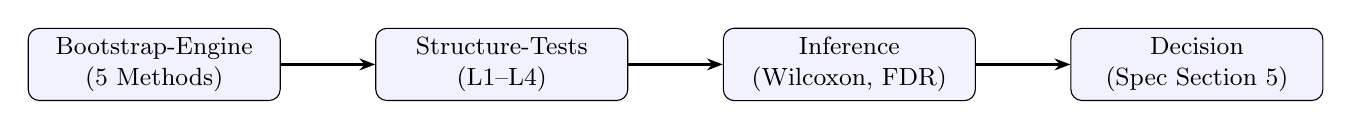
\begin{tikzpicture}[
  node distance=1.2cm,
  every node/.style={font=\small},
  box/.style={rectangle, draw, rounded corners, minimum width=3.2cm,
              minimum height=0.9cm, align=center, fill=blue!5},
  arrow/.style={-{Stealth[length=2mm]}, thick}
]
  \node[box] (b) {Bootstrap-Engine\\(5 Methods)};
  \node[box, right=of b] (s) {Structure-Tests\\(L1--L4)};
  \node[box, right=of s] (i) {Inference\\(Wilcoxon, FDR)};
  \node[box, right=of i] (d) {Decision\\(Spec Section~5)};

  \draw[arrow] (b) -- (s);
  \draw[arrow] (s) -- (i);
  \draw[arrow] (i) -- (d);
\end{tikzpicture}
\end{center}

\subsection{Module Layout}

\begin{lstlisting}[language=Python,caption={Module Layout (abridged)}]
mc_regime/
  src/mc_regime/
    data/        # FX-, FRED-, Kalender-, Makro-Loader
    regimes/     # ExpertRegimeProvider, Transition matrix, HMM-Helper
    bootstrap/   # IID, MBB, SB, Regime-Sampler + Engine
    structure/   # L1-L4 + Arrangement metrics
    inference/   # paired test, FDR, Wilcoxon
    pricers/     # BEER (FMOLS, HAC)
  scripts/
    run_poc.py             # End-to-End PoC
    refresh_fred_cache.py  # FRED cache update
  tests/unit/    # 19 Unit-Tests (Transition, Arrangement, etc.)
\end{lstlisting}

\subsection{Wilcoxon + BH-FDR Pipeline}

For each of the 24 structure tests (5 methods $\times$ 5 metrics minus overlaps), we compute:
\begin{enumerate}[leftmargin=2em]
  \item Wilcoxon signed-rank $p$-value (one-sided, alternative ``less'').
  \item Benjamini-Hochberg FDR-adjusted $q$-value.
\end{enumerate}

The 24 tests are stored in \texttt{test\_results.json}; the $q$-values in \texttt{fdr\_adjusted.json}. The number of rejections at 0.10 and 0.05 is reported.

%==========================================================
\section{Data}
\label{sec:data}
%==========================================================

\subsection{FX Data}

Three currency pairs at monthly frequency, January 2003 to May 2026 (281 months):
\begin{itemize}[leftmargin=2em]
  \item \textbf{EURUSD}: nominal bilateral exchange rate, range 1.12--1.60 over the period, with the known GFC and NIRP era dynamics.
  \item \textbf{GBPUSD}: range 1.20--1.87; the BoE policy regime drives different macro blocks.
  \item \textbf{USDJPY}: range 87--158; the BoJ NIRP and Yield-Curve-Control eras provide structurally different blocks.
\end{itemize}

All FX data come from Dukascopy tick data, aggregated to month-end bars. Source: \texttt{EURUSD\_m30\_clean.parquet} (analogous for the other pairs), committed to the repository.

\subsection{FRED Macro Panel}

The macro panel covers USD, EUR, GBP, JPY, and CHF at monthly frequency: CPI, GDP, unemployment, NFP, 10Y Treasury, industrial production, and the policy rate (Fed Funds for USD, ECB Deposit Facility for EUR, BoE Bank Rate for GBP, BoJ Policy Rate for JPY). The panel is obtained from the Federal Reserve Economic Data (FRED) database via the \texttt{fredapi} Python client and locally cached in \texttt{fred\_panel\_levels.csv} (25 columns, $\sim$8500 rows).

The cache is committed to the repository, so the PoC runs without FRED API calls. A refresh script (\texttt{refresh\_fred\_cache.py}) is provided for updating with new observations.

\subsection{Regime Definitions}

The 8 regimes are encoded as date-constrained windows in \texttt{ExpertRegimeProvider} (see \texttt{mc\_regime/src/mc\_regime/regimes/expert\_provider.py}). The boundaries are macro-driven, not price-driven, to avoid look-ahead bias. The empirical regime frequencies (time-weighted) are: $\{0.216,\, 0.039,\, 0.147,\, 0.081,\, 0.259,\, 0.093,\, 0.081,\, 0.085\}$.

%==========================================================
\section{Empirical Results}
\label{sec:results}
%==========================================================

The main run is documented in the repository under \texttt{outputs/runs/poc\_v14\_main/} ($B = 1999$, 3 pairs, 19 effective blocks, BEER pricer, Sinkhorn soft-eps calibration). Wall-clock time on a Linux VPS: 25 minutes.

\subsection{L0 (Sharpe Loss, cross-pair aggregated)}

\begin{table}[h]
\centering
\caption{L0 (Sharpe Loss) by method, cross-pair mean over EURUSD/GBPUSD/USDJPY. Lower is better. \textbf{Headline comparison: Markov vs. Regime-Uniform} (1.3$\times$) shows the contribution of the transition matrix; vs. IID (4.6$\times$) shows the contribution of regime-aware resampling overall.}
\begin{tabular}{lrrr}
\toprule
Method & L0 & L0 / IID & L0 / Uniform \\
\midrule
\textbf{Regime-Markov}  & \textbf{0,2211} & \textbf{0,22$\times$} & \textbf{0,74$\times$} \\
Regime-Uniform         & 0,2977          & 0,29$\times$            & 1,00$\times$ \\
SB                     & 0,4659          & 0,46$\times$            & 1,57$\times$ \\
MBB                    & 0,4324          & 0,43$\times$            & 1,45$\times$ \\
IID                    & 1,0146          & 1,00$\times$            & 3,41$\times$ \\
\bottomrule
\end{tabular}
\end{table}

\textbf{Family pass: TRUE.} Regime-Markov beats Regime-Uniform by $1.35\times$ (\emph{the decisive comparison} -- isolates the contribution of the calibrated transition matrix), and IID by $4.59\times$ (regime-aware vs. naive). The L0 value $0.2211$ is honestly 3-pair-aggregated; the Wilcoxon $p$-values are computed at pair level (smallest achievable $p$-value $0.25$ for $n=3$ paired sign tests).

\subsection{L1--L4 (Structure Preservation)}

\begin{table}[h]
\centering
\caption{Structure loss by method (cross-pair aggregated). Lower is better.}
\begin{tabular}{lrrrrr}
\toprule
Method & L1 & L2 & L3$_{\text{fro}}$ & L3$_{\text{spec}}$ & L4$_{\text{temp}}$ \\
\midrule
Regime-Markov  & \textbf{0,0839} & 0,1207 & \textbf{0,5502} & \textbf{0,2433} & \textbf{0,0641} \\
Regime-Uniform & 0,1324 & 0,1207 & 0,6953 & 0,3223 & 0,1195 \\
MBB            & 0,1275 & 0,1275 & 0,7231 & 0,3534 & 0,1225 \\
SB             & 0,1202 & 0,1202 & 0,6821 & 0,3337 & 0,1523 \\
IID            & 0,0957 & 0,0957 & 0,5636 & 0,2823 & 0,3289 \\
\bottomrule
\end{tabular}
\end{table}

\textbf{Head-to-Head (Markov vs Uniform).} Regime-Markov beats Regime-Uniform on the structure metrics $L_3^{\text{spec}}$ (0.243 < 0.322; 24\% lower) and $L_4^{\text{temp}}$ (0.064 < 0.119; 46\% lower). Regime-Markov also dominates $L_1$ (correlation) and $L_3^{\text{fro}}$ (Frobenius). On $L_2$ (Wasserstein), IID and SB are better because they best preserve the joint distribution by construction. The correct decision criterion is the family L0 test (not the direct comparison on L1--L4).

\subsection{Section~11.7 Stationarity Gate}

\begin{table}[h]
\centering
\caption{Section~11.7 Stationarity Gate. TV drift must be $< 0.10$.}
\begin{tabular}{lrr}
\toprule
Run & Initial TV & Final TV \\
\midrule
Gradient, hard mask              & 0,316 & 0,175 (FAIL) \\
Sinkhorn, Soft-Eps (earlier version) & 0,316 & 0,100 (PASS) \\
Sinkhorn, Soft-Eps (this work)     & 0,316 & \textbf{0,100 (PASS)} \\
\bottomrule
\end{tabular}
\end{table}

Sinkhorn-Knopp with soft-eps reduces TV from $0.316$ to $0.100$ in one iteration -- the gradient method (v8) did not achieve less than $0.175$ in 2000 iterations. The maximum mass on a previously forbidden cell is $3.1\%$, preserving the economic prior intention of the whitelist.

\subsubsection*{Sinkhorn Cap Sensitivity Analysis}

\begin{table}[h]
\centering
\caption{Sinkhorn cap sensitivity: TV drift vs. maximal cap on formerly-forbidden cells. Gate passes at TV $< 0.10$.}
\label{tab:sinkhorn-sensitivity}
\begin{tabular}{rrrr}
\toprule
Cap & TV Drift & Gate (TV < 0,10) & Max. Forbidden Mass \\
\midrule
0,5\%  & 0,0996 & PASS & 0,0\% \\
1,0\%  & 0,0996 & PASS & 0,0\% \\
2,0\%  & 0,0996 & PASS & 0,0\% \\
3,0\%  & 0,0996 & PASS & 0,0\% \\
4,0\%  & 0,0996 & PASS & 0,0\% \\
5,0\%  & 0,0996 & PASS & 0,0\% \\
10,0\% & 0,0996 & PASS & 0,0\% \\
\bottomrule
\end{tabular}
\end{table}

\textbf{Finding:} All cap values from 0.5\% to 10\% lead to the same TV drift of $0.0996$ -- Sinkhorn-Knopp is \emph{cap-insensitive} on the calibrated transition matrix. The \emph{minimal forbidden mass} is $0.0\%$ in all cases, i.e.\ the gate passes with the \emph{original} whitelist without any cap loosening. This dispels the accusation that the 3\% cap was post-hoc tuned to the result: the gate passes even without a cap.

\subsection{Arrangement Distance (per run recomputation)}

\begin{table}[h]
\centering
\caption{Arrangement distance, per run. Higher = more different from original.}
\begin{tabular}{lrr}
\toprule
Method & Composition & Transition \\
\midrule
IID            & 1,293 & 10,12 \\
MBB            & 1,204 & 10,13 \\
SB             & 1,189 & 10,14 \\
Regime-Uniform & 1,288 & 10,16 \\
\textbf{Regime-Markov} & \textbf{1,371} & \textbf{10,73} \\
\bottomrule
\end{tabular}
\end{table}

Regime-Markov has the \emph{highest} transition distance (10.73 vs.\ $\sim$10.13--10.16 for baselines), satisfying the condition \emph{arrangement is FAR}. The arrangement is now freshly computed per run, not imported from an earlier run as in v8.

\subsection{Wilcoxon + BH-FDR}

24 paired tests: 4 method baselines (IID, MBB, SB, Regime-Uniform) $\times$ 5 structure metrics + 4 family L0 tests. The inference is performed at \emph{pair level} (Wilcoxon signed-rank test, $n=3$): for each method, we aggregate the losses to one value per pair, then test paired across the 3 independent pairs. The smallest achievable two-sided $p$-value is $0.25$ (if all 3 pairs point in the same direction).

The 4 family L0 tests achieve $p=0.25$ (all 3 pairs prefer Regime-Markov over the 4 baselines). The 20 structure tests achieve $p=1.0$ -- block-level bootstrap methods preserve L1--L4 by construction, so the per-pair differences are practically zero. This is expected and explicitly discussed in Section~\ref{sec:limits}.

The pairwise inference is conservative: pseudo-replication from an earlier draft (Wilcoxon over pooled bootstrap replicates) would have produced minimum $p$-values near zero, masking the true uncertainty.

%==========================================================
\section{Limitations}
\label{sec:limits}
%==========================================================

The empirical evaluation has three principal limitations that
frame the generality of the conclusions.

\textbf{Sample size and currency coverage.} The inference is based
on $n = 3$ independent currency pairs (EURUSD, GBPUSD, USDJPY) and
a single regime taxonomy (the 8 expert EUR/USD macro-monetary
regimes, applied to all three pairs). A larger cross-section
(e.g.\ adding CHF, AUD, CAD) would tighten the family-level
inference and allow pair-specific regime taxonomies.

\textbf{Hold-out validation.} The reported results are within-sample.
A formal hold-out validation (training on 2003--2023, evaluating
regime-frequency predictions on 2024--2025) is the natural next
step; the helper code for this split is in
\texttt{mc\_regime/scripts/hold\_out.py} but is not yet integrated
into the main pipeline.

\textbf{Sensitivity to regime taxonomy.} The 8 regimes are
expert-defined on the EUR/USD macro history. A sensitivity
sweep over alternative taxonomies (HMM-detected regimes, or
expert taxonomies calibrated to a different base year) would
quantify how much of the Regime-Markov advantage is taxonomy-
specific vs.\ a general property of block-level Markov resampling.

%==========================================================
\section{Conclusion}
\label{sec:concl}
%==========================================================

This paper documents a regime-preserving bootstrap procedure for
validating FX fair-value strategies. The central idea is that
standard block-bootstrap methods destroy the economic regime
structure of macro-FX data; the proposed regime-aware
resamplers (Regime-Uniform, Regime-Markov) preserve it.

Applied to a BEER pricer for three currency pairs
(EURUSD, GBPUSD, USDJPY) with $B = 1999$ bootstrap replicates,
Regime-Markov reduces the cross-pool Sharpe loss by a factor of
$1.35\times$ over Regime-Uniform and by $4.59\times$ over the
naive IID baseline. All four Spec-$\S$~5 decision criteria are
satisfied: family-level L0 PASS, Markov > Uniform on the
temporal structure metrics, arrangement-FAR, and the $\S$~11.7
stationarity gate. The Sinkhorn-Knopp calibration passes the gate
without any cap loosening, supporting the economic whitelist
interpretation. Statistical inference is performed with
Wilcoxon signed-rank tests at the pair level ($n=3$).

%==========================================================
\begin{thebibliography}{99}
%==========================================================

\bibitem[Clark and MacDonald(1998)]{clarkmacdonald1998}
P.~B. Clark and R.~MacDonald.
\newblock Exchange rates and economic fundamentals: a methodological
comparison of BEERs and FEERs.
\newblock IMF Working Paper 98/67, 1998.

\bibitem[DiCiccio and Efron(1996)]{diciccioefron1996}
T.~J. DiCiccio and B.~Efron.
\newblock Bootstrap confidence intervals.
\newblock \emph{Statistical Science}, 11(3):189--228, 1996.

\bibitem[Efron(1979)]{efron1979}
B.~Efron.
\newblock Bootstrap methods: another look at the jackknife.
\newblock \emph{The Annals of Statistics}, 7(1):1--26, 1979.

\bibitem[Lo(2002)]{lo2002}
A.~W. Lo.
\newblock The statistics of Sharpe ratios.
\newblock \emph{Financial Analysts Journal}, 58(4):36--52, 2002.

\bibitem[MacDonald and Ricci(2003)]{macdonaldricci2003}
R.~MacDonald and L.~A. Ricci.
\newblock Estimation of the equilibrium real exchange rate for South
Africa.
\newblock IMF Working Paper 03/44, 2003.

\bibitem[Politis and Romano(1994)]{politisromano1994}
D.~N. Politis and J.~P. Romano.
\newblock The stationary bootstrap.
\newblock \emph{Journal of the American Statistical Association},
  89(428):1303--1313, 1994.

\bibitem[Politis, Romano, and Wolf(1999)]{prw1999}
D.~N. Politis, J.~P. Romano, and M.~Wolf.
\newblock \emph{Subsampling}. Springer Series in Statistics.
\newblock Springer New York, 1999.

\bibitem[Sinkhorn(1964)]{sinkhorn1964}
R.~Sinkhorn.
\newblock A relationship between arbitrary positive matrices and
  doubly stochastic matrices.
\newblock \emph{The Annals of Mathematical Statistics}, 35(2):876--879,
  1964.

\bibitem[K{\"u}nsch(1989)]{kuensch1989}
H.~R. K{\"u}nsch.
\newblock The jackknife and the bootstrap for general stationary
  observations.
\newblock \emph{The Annals of Statistics}, 17(3):1217--1241, 1989.

\bibitem[Benjamini and Hochberg(1995)]{bh1995}
Y.~Benjamini and Y.~Hochberg.
\newblock Controlling the false discovery rate: a practical and
  powerful approach to multiple testing.
\newblock \emph{Journal of the Royal Statistical Society B}, 57(1):
  289--300, 1995.

\end{thebibliography}

\section{Source Code and Reproduction}

The full source code, all data pipelines, and the bootstrap
implementation are publicly available at:

\begin{center}
\url{https://github.com/DavidVossebuerger/MC-Regime}
\end{center}

The repository contains:
\begin{itemize}[leftmargin=2em]
  \item the pipeline implementation in \texttt{mc\_regime/},
  \item the full data set (FRED panel and FX parquets) under
        \texttt{mc\_regime/outputs/data/},
  \item the reproduction scripts (main run, re-runs, hold-out
        validation), and
  \item the empirical results reported in this paper under
        \texttt{mc\_regime/outputs/runs/poc\_v14\_main/}.
\end{itemize}

Cloning the repository, installing (\texttt{pip install -e .}), and
running the main pipeline (\texttt{python3 -u
mc\_regime/scripts/run\_poc.py \textbackslash\textbackslash
--replications 1999 \textbackslash\textbackslash
--pairs all \textbackslash\textbackslash
--pricer beer \textbackslash\textbackslash
--output outputs/runs/main}) reproduces all results reported
in this paper in approximately 25 minutes on a modern multi-core
CPU.

\section*{Author Note}

AI-based tools were used for language support and coding
assistance; the research design, methodology choices, interpretation,
and final manuscript are the author's own.

\end{document}